\chapter{Código sistema de usuários}

Neste apêndice encontra-se algumas partes importantes do código do Sistema de Usuários. O código inteiro pode ser baixado no \textit{link}: \url{https://github.com/CamiloAvelar/user-service}

\begin{figure}[htbp]
	\centering
	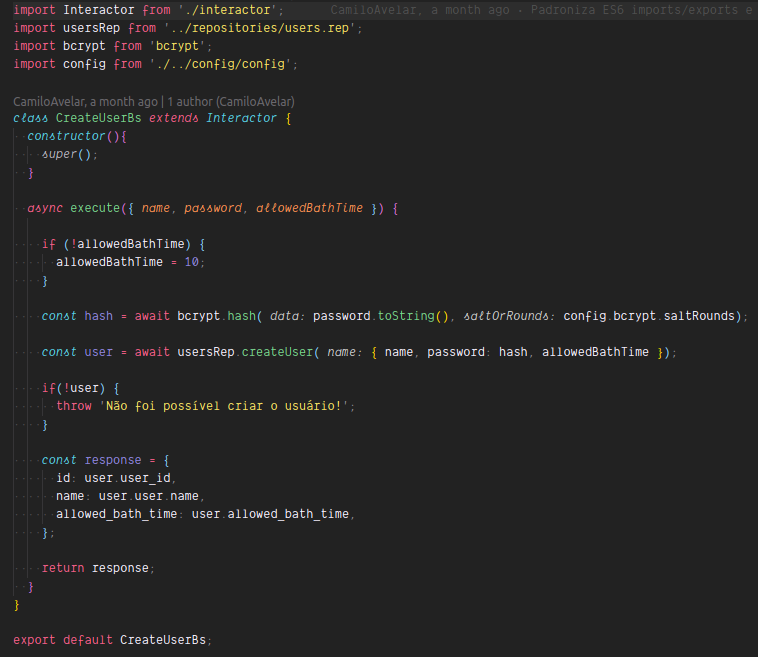
\includegraphics[width=1\linewidth]{figuras/userservice/createuser.png}
	\caption{Código para criar usuário}
	\label{fig:createuser}
\end{figure}

\begin{figure}[htbp]
	\centering
	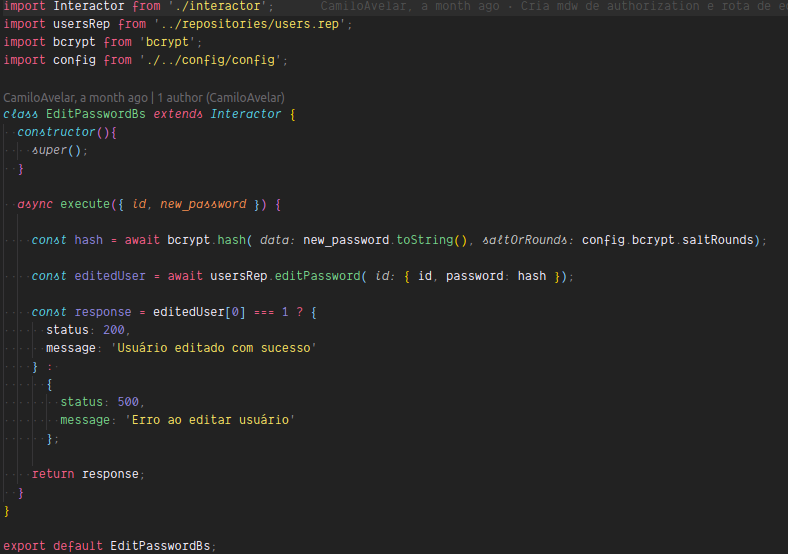
\includegraphics[width=1\linewidth]{figuras/userservice/editpassword.png}
	\caption{Código para editar senha do usuário}
	\label{fig:editpass}
\end{figure}

\begin{figure}[htbp]
	\centering
	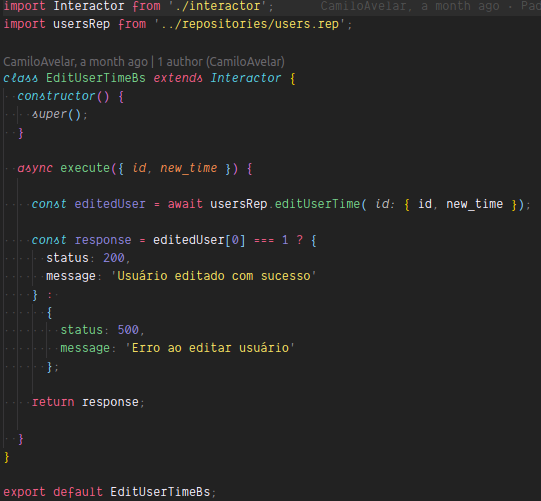
\includegraphics[width=1\linewidth]{figuras/userservice/edittime.png}
	\caption{Código para editar tempo do usuário}
	\label{fig:edittime}
\end{figure}

\begin{figure}[htbp]
	\centering
	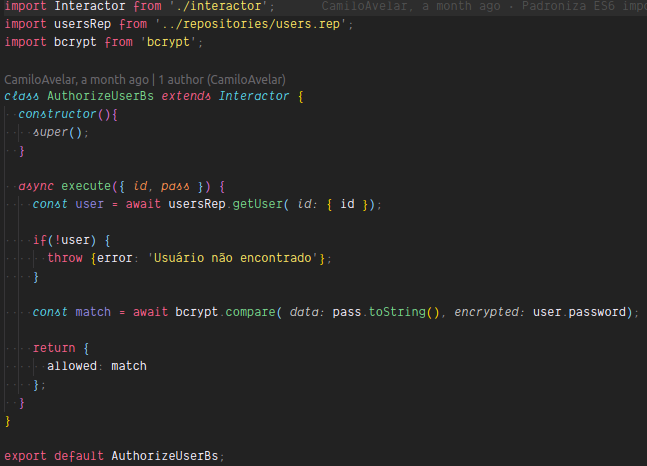
\includegraphics[width=1\linewidth]{figuras/userservice/authorizeuser.png}
	\caption{Código para autorizar usuário}
	\label{fig:autorizar}
\end{figure}

\begin{figure}[htbp]
	\centering
	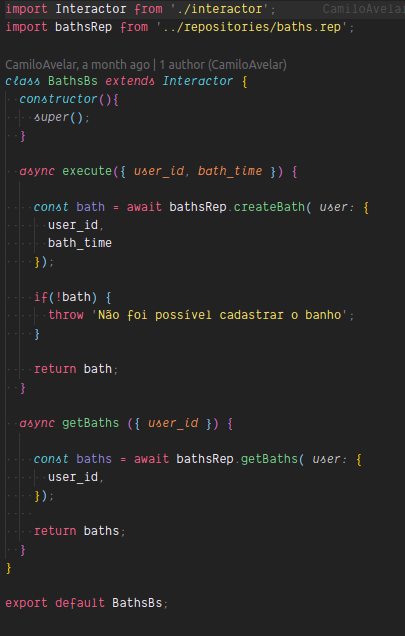
\includegraphics[width=1\linewidth]{figuras/userservice/baths.png}
	\caption{Código para cadastrar banho do usuário}
	\label{fig:cadastra-banho}
\end{figure}

\begin{figure}[htbp]
	\centering
	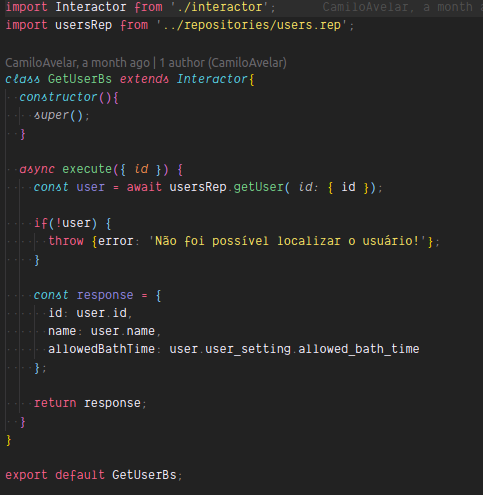
\includegraphics[width=1\linewidth]{figuras/userservice/getuser.png}
	\caption{Código para recuperar usuários}
	\label{fig:getuser}
\end{figure}

\chapter{Código sistema de comunicação MQTT}

Neste apêndice encontra-se algumas partes importantes do código do Sistema de comunicação. O código inteiro pode ser baixado no \textit{link}: \url{https://github.com/CamiloAvelar/mqtt-logger-service}

\begin{figure}[htbp]
	\centering
	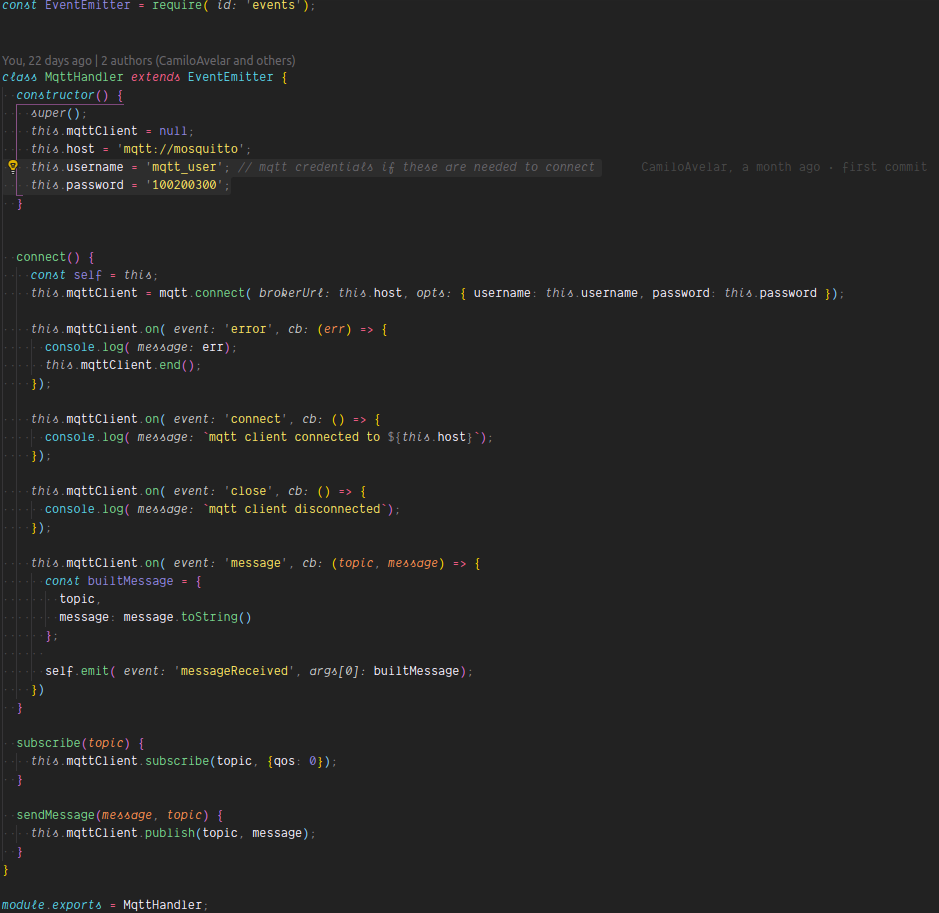
\includegraphics[width=1\linewidth]{figuras/mqttlogger/mqtt.png}
	\caption{Código para comunicação mqtt}
	\label{fig:mqtt}
\end{figure}

\begin{figure}[htbp]
	\centering
	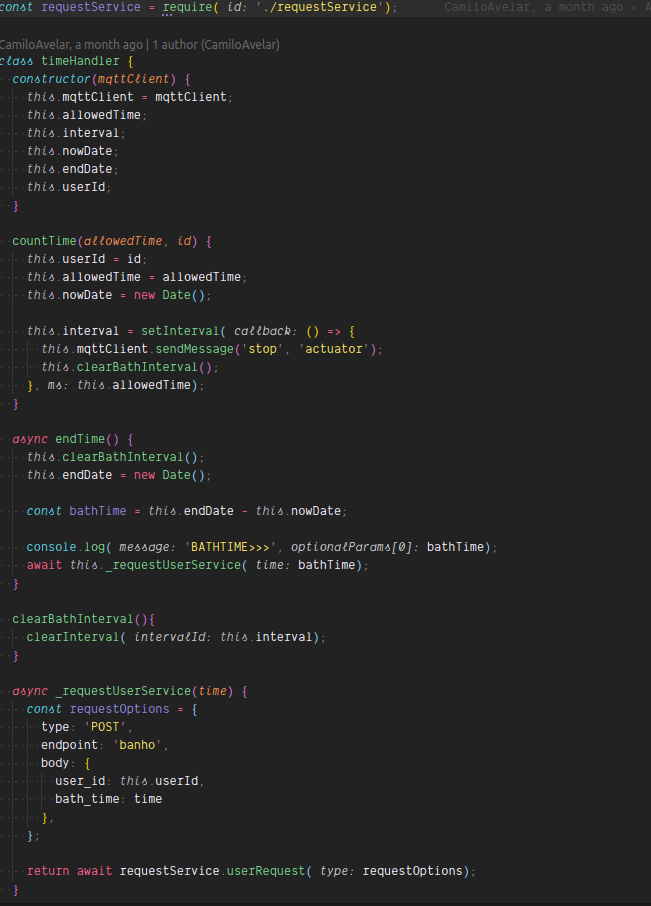
\includegraphics[width=1\linewidth]{figuras/mqttlogger/time.png}
	\caption{Código que lida com o tempo do banho}
	\label{fig:time}
\end{figure}

\begin{figure}[htbp]
	\centering
	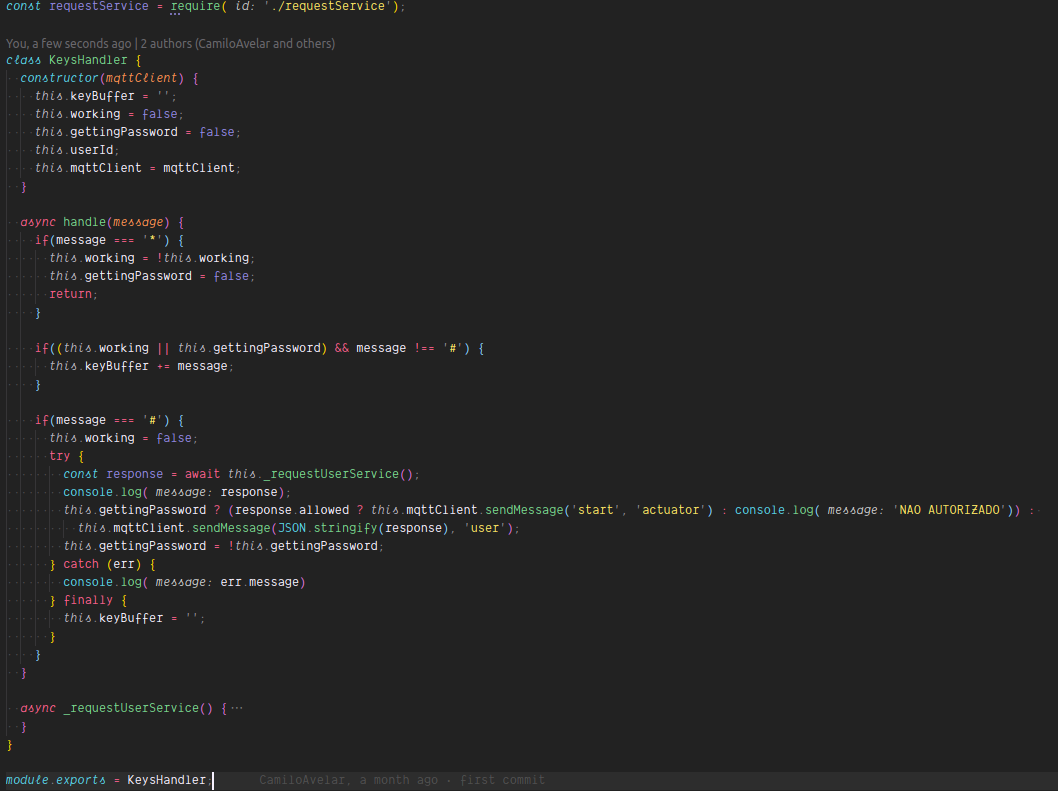
\includegraphics[width=1\linewidth]{figuras/mqttlogger/keystopic.png}
	\caption{Código que lida com as teclas apertadas no teclado numérico}
	\label{fig:keys}
\end{figure}

\begin{figure}[htbp]
	\centering
	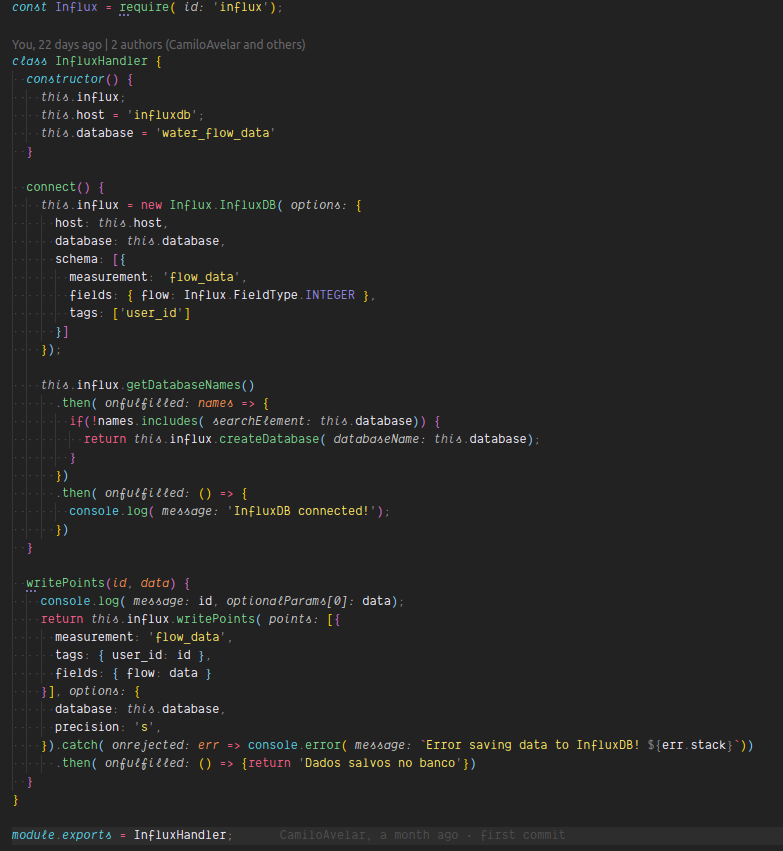
\includegraphics[width=1\linewidth]{figuras/mqttlogger/influx.png}
	\caption{Código que lida com a comunicação com o InfluxDB}
	\label{fig:influx}
\end{figure}

\chapter{Docker-compose.yml}

\begin{lstlisting}[language=Python]
version: "3.5"

services:
	user:
		build: ./user-service
		command: gulp
		depends_on:
			- postgres
		volumes:
			- ./user-service:/app
		ports:
			- "3001:3001"
		networks:
			- default

	mqtt-logger:
		build: ./mqtt-logger
		command: npm start
		depends_on:
			- mosquitto
		volumes:
			- ./mqtt-logger:/app
		ports:
			- "3002:3002"

	postgres:
		image: postgres
		restart: always
		environment:
		POSTGRES_USER: pi
		POSTGRES_PASSWORD: 100200300
		POSTGRES_DB: postgres
		CONFIGS: "listen_addresses:'*'"
		volumes:
			- ./postgres/data:/var/lib/postgresql/data
		expose:
			- "5432"
		ports:
			- "5432:5432"
		networks:
			- default

	migration:
		image: src_user:latest
		command: ["./wait-for-it/wait-for-it.sh", "postgres:5432", "--", "npm", "run", "migrate"]
		links:
			- postgres
		depends_on:
			- postgres

	homeassistant:
		container_name: homeassistant
		restart: unless-stopped
		image: homeassistant/home-assistant
		volumes:
			- ./homeassistant:/config
		depends_on:
			- mosquitto
		network_mode: host
		privileged: true
		expose:
			- "8123"
		ports:
			- "8123:8123"

	influxdb:
		image: influxdb:latest
		container_name: influxdb
		restart: always
		ports:
			- "8083:8083"
			- "8086:8086"
			- "8090:8090"
		volumes:
			# Data persistency
			# sudo mkdir -p /srv/docker/influxdb/data
			- ./influxdb/data:/var/lib/influxdb

	grafana:
		image: grafana/grafana
		container_name: grafana
		restart: always
		ports:
			- "3003:3000"
		links:
			- influxdb
		volumes:
			# Data persistency
			# sudo mkdir -p /srv/docker/grafana/data; chown 472:472 /srv/docker/grafana/data
			- ./grafana/data:/var/lib/grafana
	
	mosquitto:
		image: eclipse-mosquitto
		hostname: mosquitto
		container_name: mosquitto
		restart: always
		user: 1883:1883
		expose:
			- "1883"
			- "9001"
		ports:
			- "1883:1883"
			- "9001:9001"
		volumes:
			- ./mosquitto/config:/mosquitto/config
			# sudo chown 1883:1884 /mosquitto/logs
			- ./mosquitto/logs:/mosquitto/logs
		networks:
			- default
		networks:
		default:
		driver: bridge
		ipam:
		config:
			- subnet: 172.18.1.0/24
\end{lstlisting}